\chapter{User Manual}
\label{usermanual}
%In the user manual you should explain, step-by-step, how to reproduce the demo that you showed in the oral presentation or the results you mentioned in the previous chapters.\\ If it is necessary to install some toolchain that is already well described in the original documentation (i.e., Espressif's toolchain for ESP32 boards or the SEcube toolchain) just insert a reference to the original documentation (and remember to clearly specify which version of the original documentation must be used). There is no need to copy and paste step-by-step guides that are already well-written and available.\\The user manual must explain how to re-create what you did in the project, no matter if it is low-level code (i..e VHDL on SEcube's FPGA), high-level code (i.e., a GUI) or something more heterogeneous (i.e. a bunch of ESP32 or Raspberry Pi communicating among them and interacting with other devices).  



\section {SEcube™ Software Development Kit (version 1.5.2)}
Copyright (C) 2021 Blu5 Labs Ltd.

\section {Licence}
All SEcube releases published on this website are Open Source - GPL 3.0 and are developed by the Academia Community.

\section {Terms of use}
By downloading the software from this page, you agree to the specified terms.

The software is provided to you "as is" and we make no express or implied warranties whatsoever with respect to its functionality, operability, or use, including, without limitation, any implied warranties of merchantability, fitness for a particular purpose, or infringement. We expressly disclaim any liability whatsoever for any direct, indirect, consequential, incidental or special damages, including, without limitation, loss revenues, lost profits, losses resulting from business interruption or loss of data, regardless of the form of action or legal thereunder which the liability may be asserted, even if advised of the possibility likelihood of such damages.

\section {PUF}
This is a project made for the course of Cybersecurity for embedded systems of the Masters on embedded system in Politecnico di Torino.

The purpose of this project is to extract the RAM PUFs from the memory of the SEcube storing them on a DB, in this case a simple txt file, and perform also a challenge on the board.

\section {Instructions to run the project}

\subsection {Import the project}
Instructions on how to import the project are the same as the ones for the original project provided in the wiki

\subsection {Run the project}
the steps to run the project are the following


\begin{itemize}
\item {Erase the flash memory of the SEcube}

\begin{figure}[H]
\centering
  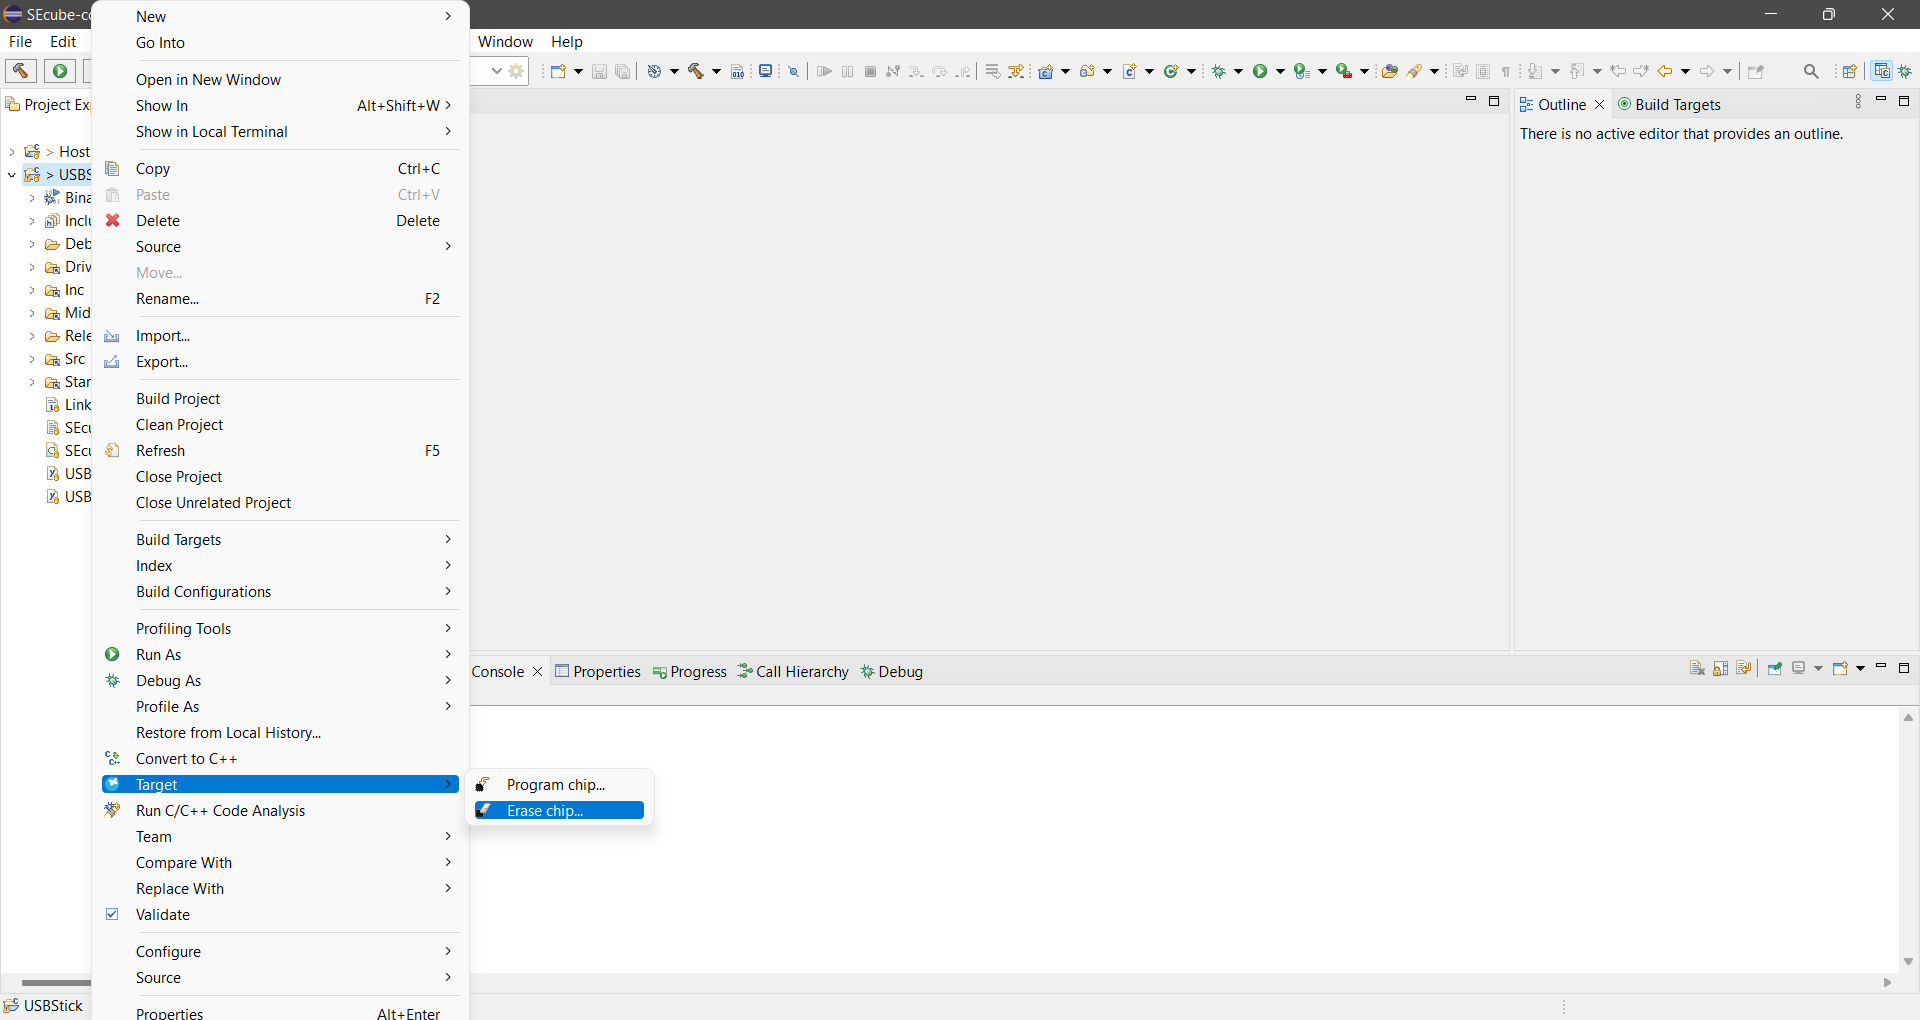
\includegraphics[width=5cm]{../../images/erase_flash.png}
  \caption{Erase flash}
  \label{fig:Erase flash}
\end{figure}
%![erase_flash]

\item {Flash the SEcube}
\begin{figure}[H]
\centering
  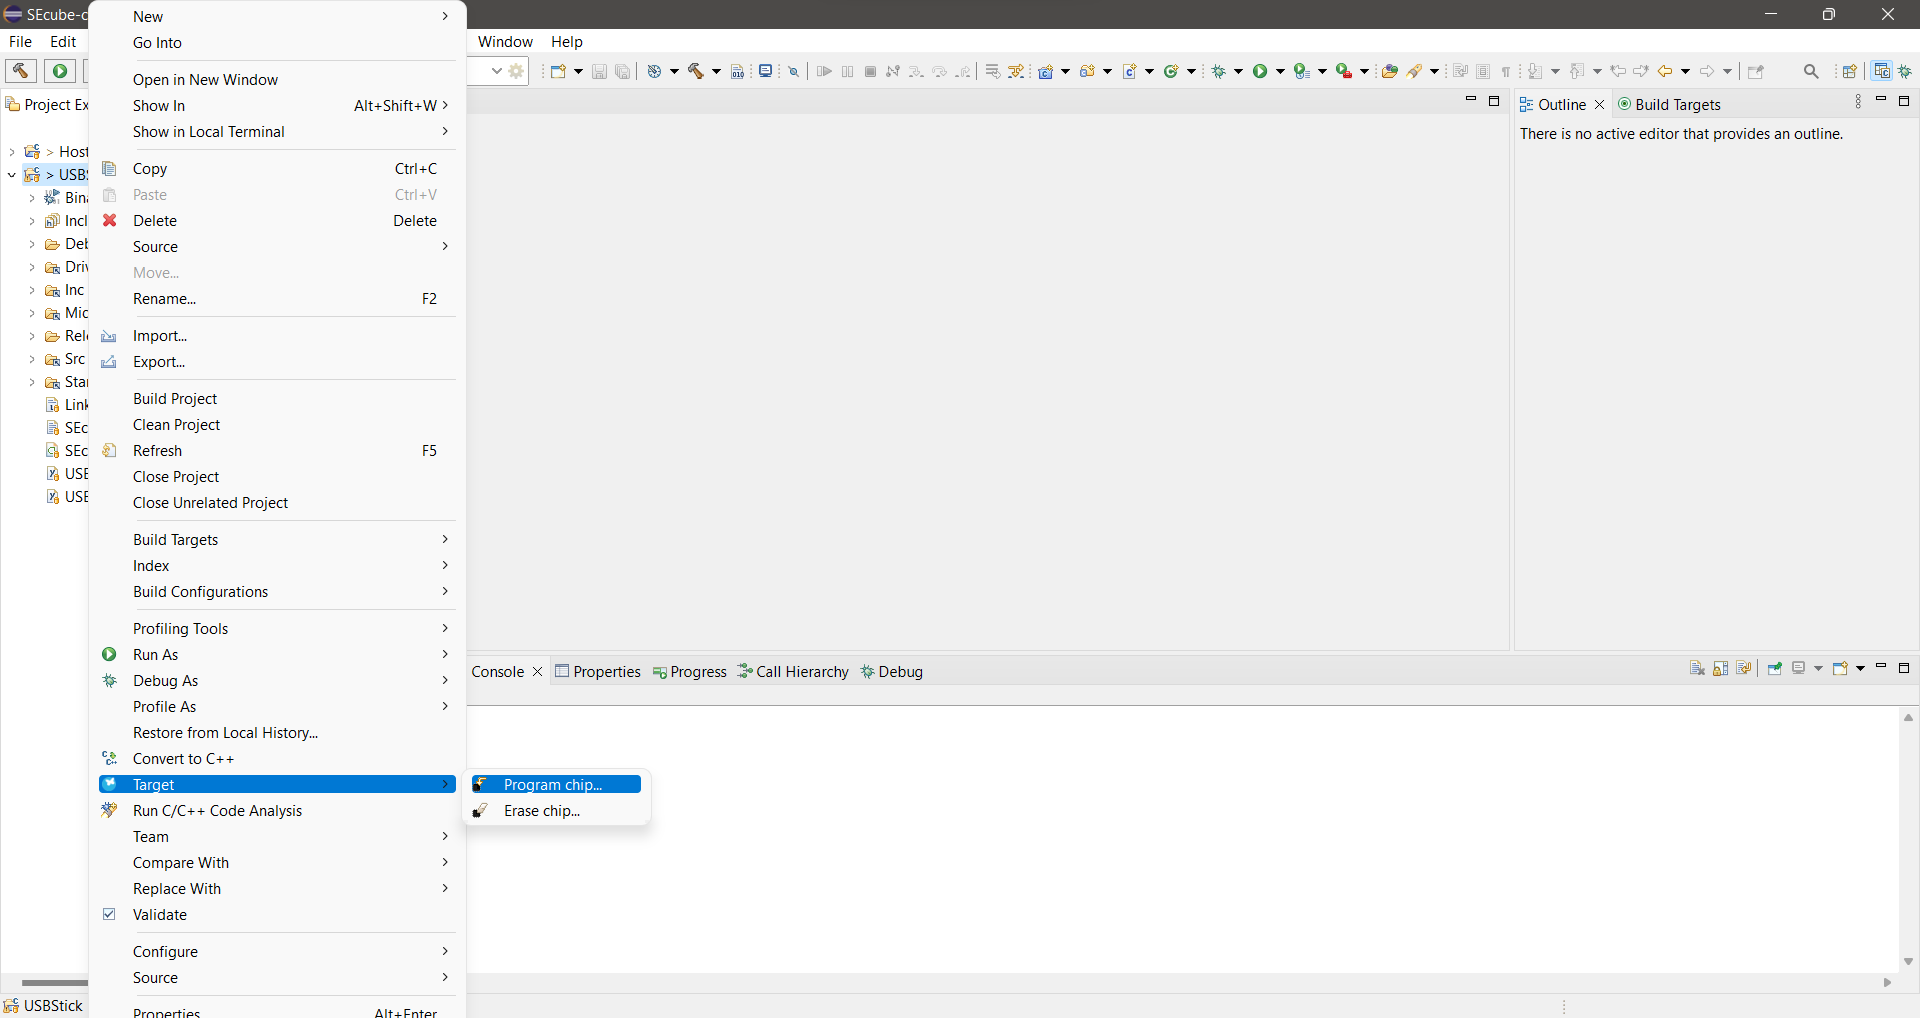
\includegraphics[width=5cm]{../../images/chip_flash.png}
  \caption{Chip flash}
  \label{fig:Chip flash}
\end{figure}

%![chip_flash]

\item {Run on the host the "puf\_db\_init.cpp"}
\begin{figure}[H]
\centering
  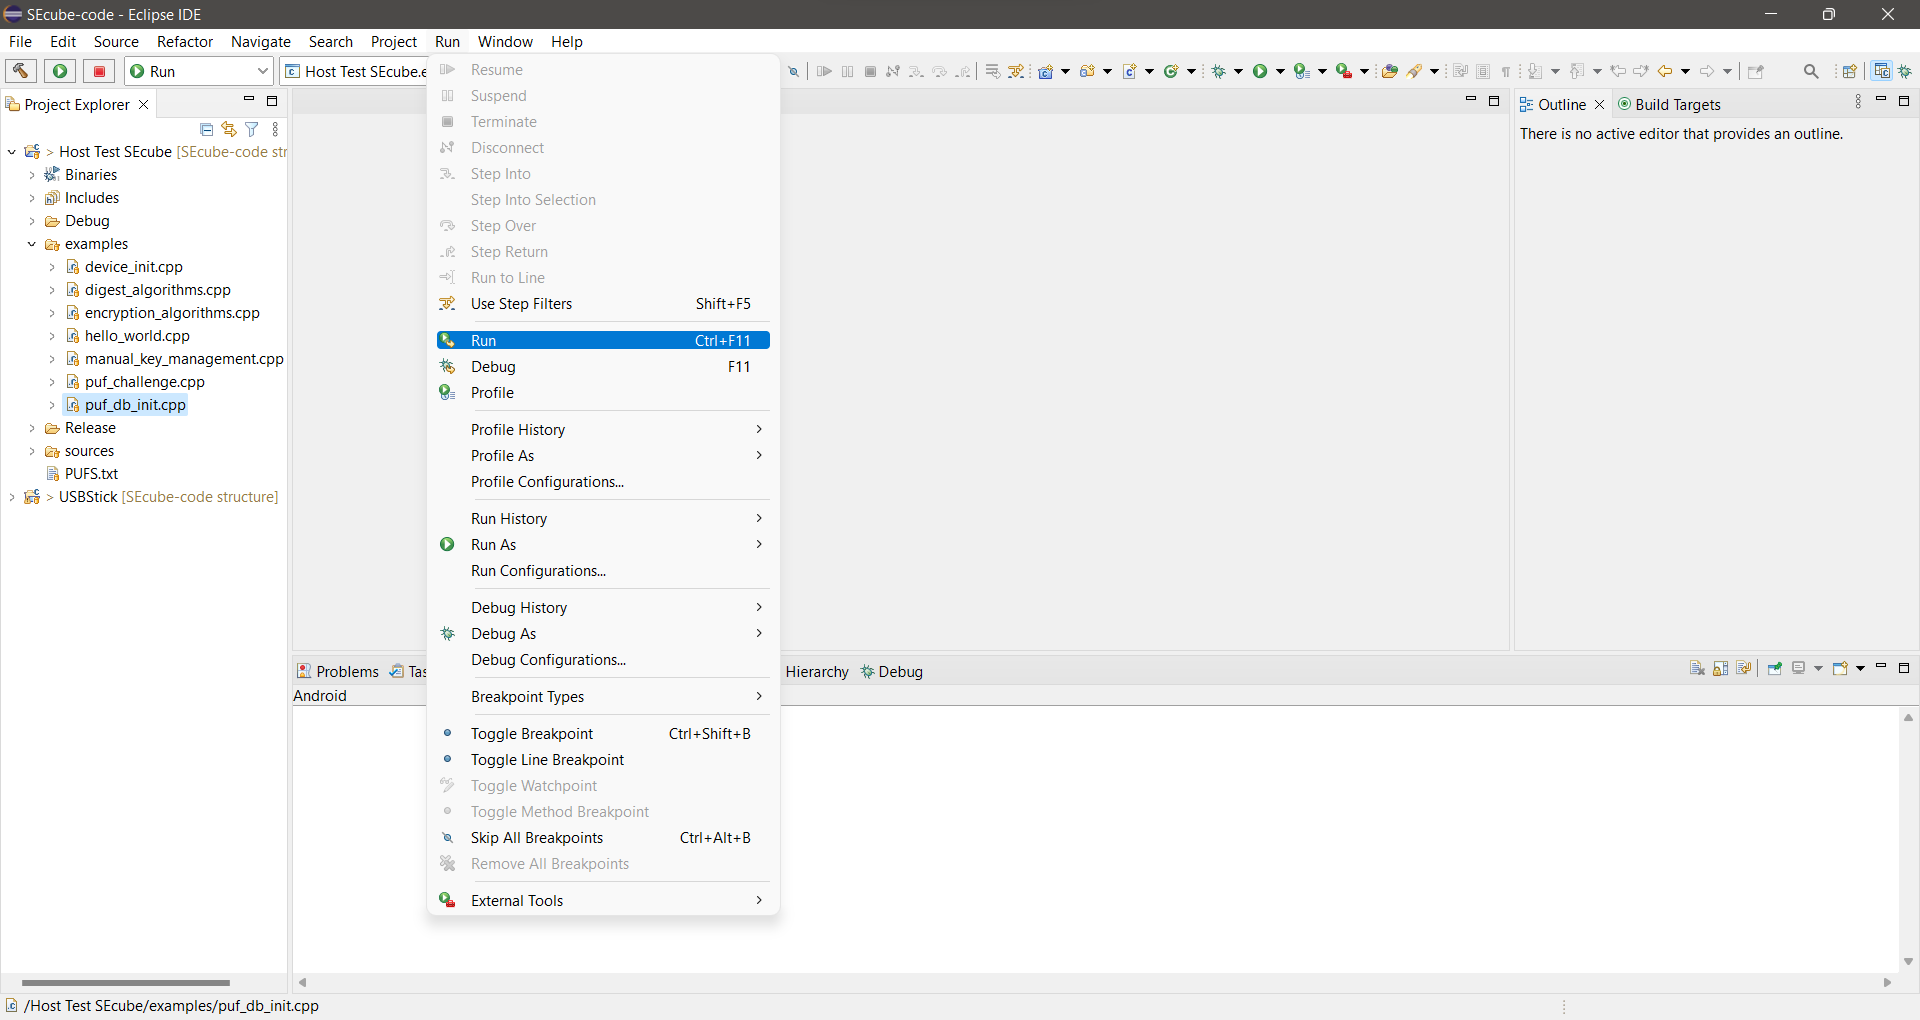
\includegraphics[width=5cm]{../../images/puf_db_init.png}
  \caption{Puf db init}
  \label{fig:Puf db init}
\end{figure}
%![puf_db_init]

\item {Run on the host the "puf\_challenge.cpp"}
\begin{figure}[H]
\centering
  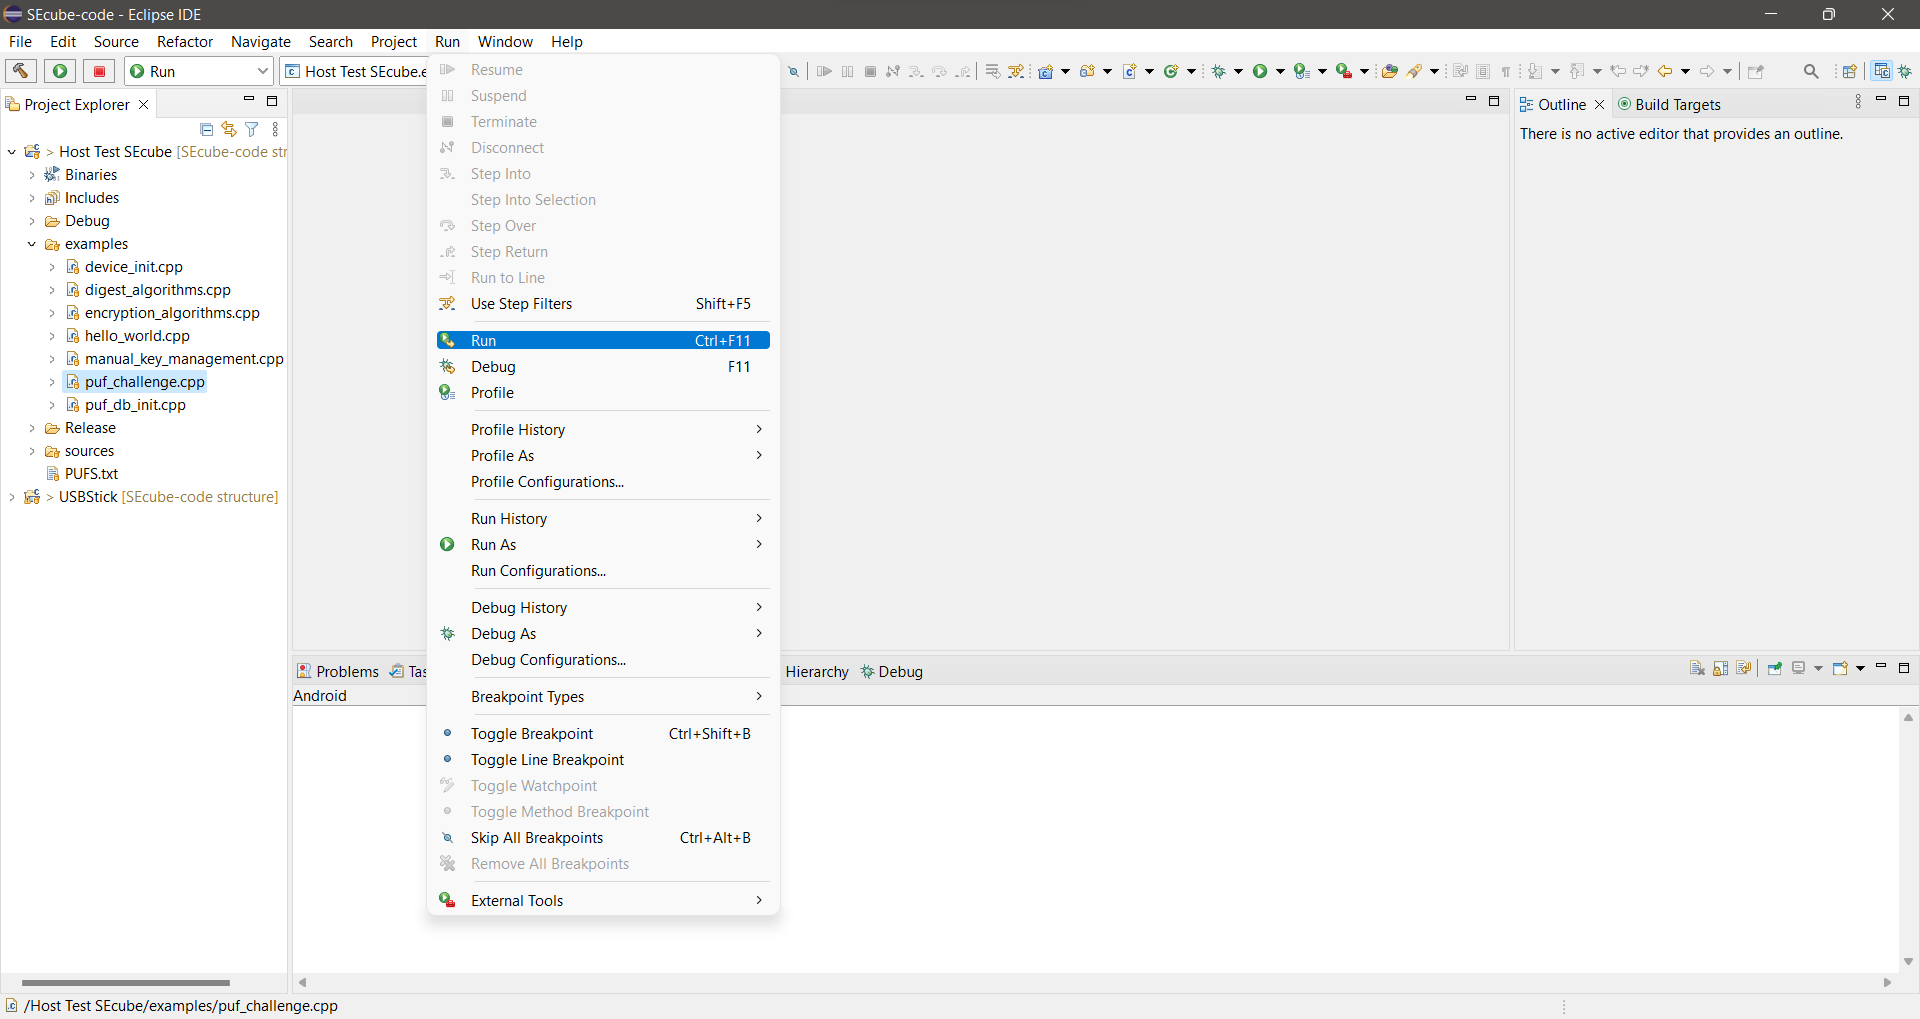
\includegraphics[width=5cm]{../../images/puf_challenge.png}
  \caption{Puf challenge}
  \label{fig:Puf challenge}
\end{figure}
%![puf_challenge]

\end{itemize}




